%% Author: Leighton Pritchard
%% Copyright: James Hutton Institute
%% 2014-11-21: Slides for teaching at University of Strathclyde, 21st November 2014
%% This presentation was an invited guest lecture on microbial genomics and bioinformatics
%% for the BM405 course.

%% UNCOMMENT FOR SLIDES
\documentclass[table]{beamer}
\mode<presentation>

%% UNCOMMENT FOR HANDOUTS
%\documentclass[handout]{beamer}
\usepackage{handoutWithNotes}
\pgfpagesuselayout{4 on 1 with notes}[a4paper,border shrink=5mm]

%% GENERIC STYLE SETTINGS BELOW
\usetheme{default}
\usepackage{listings}
\usepackage{multirow}
\usepackage{xcolor}
\usepackage{hyperref}

\usebackgroundtemplate{

\includegraphics[width=\paperwidth,height=\paperheight]{images/hutton_background}
}
%% PRESENTATION CONFIGURATION PARAMETERS %%%%%%%%%%%%%%%%%%%%%%%%%%%%%%%%%%%%%%%
%\titlebackgroundfile{images/hutton_title}
%\framebackgroundfile{images/hutton_background}
\definecolor{hutton_green}{HTML}{78A22F}
\definecolor{hutton_purple}{HTML}{872175}
\definecolor{hutton_blue}{HTML}{569BBE}
\usefonttheme{structurebold}
\setbeamercolor{alerted text}{fg=orange}
\setbeamercolor{background canvas}{bg=white}
\setbeamercolor{block title}{bg=hutton_purple}
\setbeamercolor{frametitle}{fg=hutton_purple}
\setbeamercolor{title}{fg=black}
\setbeamercolor{titlelike}{fg=hutton_green}
\setbeamercolor{author}{fg=hutton_purple}
\setbeamercolor{author in head/foot}{fg=white}
\setbeamercolor{title in head/foot}{fg=white}
\setbeamercolor{section in head/foot}{fg=hutton_purple}
\setbeamercolor{normal text}{fg=black}
\setbeamercolor{frametitle}{fg=hutton_purple}
\setbeamerfont{block title}{size={}}
\setbeamerfont{author}{size=\footnotesize}
\setbeamerfont{institute}{size=\tiny}
\setbeamerfont{date}{size=\footnotesize}
\setbeamercolor{section in toc shaded}{fg=hutton_purple}
\setbeamercolor{section in toc}{fg=hutton_purple}
\setbeamercolor{subsection in toc shaded}{fg=hutton_purple}
\setbeamercolor{subsection in toc}{fg=hutton_purple}
\setbeamertemplate{itemize item}[circle]
\setbeamertemplate{itemize subitem}[circle]
\setbeamertemplate{itemize subsubitem}[circle]
\setbeamertemplate{itemize subsubsubitem}[circle]
\setbeamercolor{itemize item}{fg=hutton_purple}
\setbeamercolor{itemize subitem}{fg=hutton_purple}
\setbeamercolor{itemize subsubitem}{fg=hutton_purple}
\setbeamercolor{itemize subsubsubitem}{fg=hutton_purple}
\setbeamercolor{enumerate item}{fg=hutton_purple}
\setbeamercolor{enumerate subitem}{fg=hutton_purple}
\setbeamercolor{enumerate subsubitem}{fg=hutton_purple}
\setbeamercolor{enumerate subsubsubitem}{fg=hutton_purple}
\setbeamercolor{alerted text}{fg=hutton_green}
\setbeamerfont{alerted text}{series=\bfseries}
% This command makes sure that acrobat reader doesn't change the colours of the slide
% when there are figures with transparencies.
\pdfpageattr {/Group << /S /Transparency /I true /CS /DeviceRGB>>}

%Disables discrete bottom navigation bar
%\beamertemplatenavigationsymbolsempty

% Modify the slide titles to avoid the corner images,
\setbeamertemplate{frametitle}
{
\vspace{0.05\textheight}
\noindent\quad\begin{minipage}[t][0.12\textheight][t]{0.85\textwidth}
\insertframetitle\par
\end{minipage}
}

% Modify title page to avoid the big logo on right
\setbeamertemplate{title page}{
    \begin{picture}(0,0)
            %This ends up on top of the default background image, rather than replacing it:
            \put(-30,-165){%
                
\includegraphics[width=\paperwidth,height=\paperheight]{images/hutton_title}
            }
            \put(0,-75){%
                \begin{minipage}[b][0.4\textheight][t]{0.75\textwidth}
                    \usebeamerfont{title}\usebeamercolor[fg]{title}{\inserttitle\par}
                    \usebeamerfont{subtitle}\usebeamercolor[fg]{subtitle}{\insertsubtitle\par}
                \end{minipage}
            }
            \put(0,-125){%
                \begin{minipage}[b][0.1\textheight][t]{\textwidth}
                    \usebeamerfont{author}\usebeamercolor[fg]{author}{\insertauthor\par}
                    \usebeamerfont{institute}\usebeamercolor[fg]{institute}{\insertinstitute\par}
                \end{minipage}
            }
    \end{picture}
}

%%%%%%%%%%%%%%%%%%%%%%%%%%%%%%%%%%%%%%%%%%%%%%%%%%%%%%%%%%%%%%%%%%%%%%%%%%%%%%%%

% LISTINGS SETTING
% Settings for code listings in lstlistings

\definecolor{hutton_lightgreen}{HTML}{C8F27F}

\lstset{ %
  backgroundcolor=\color{hutton_lightgreen},   % choose the background color; you must add \usepackage{color} or \usepackage{xcolor}
  basicstyle=\tiny\ttfamily,        % the size of the fonts that are used for the code
  breakatwhitespace=false,         % sets if automatic breaks should only happen at whitespace
  breaklines=true,                 % sets automatic line breaking
  captionpos=b,                    % sets the caption-position to bottom
  commentstyle=\color{red},    % comment style
  deletekeywords={...},            % if you want to delete keywords from the given language
  escapeinside={\%*}{*)},          % if you want to add LaTeX within your code
  extendedchars=true,              % lets you use non-ASCII characters; for 8-bits encodings only, does not work with UTF-8
  frame=single,                    % adds a frame around the code
  keepspaces=true,                 % keeps spaces in text, useful for keeping indentation of code (possibly needs columns=flexible)
  keywordstyle=\color{blue},       % keyword style
%  language=Octave,                 % the language of the code
  morekeywords={*,...},            % if you want to add more keywords to the set
  numbers=left,                    % where to put the line-numbers; possible values are (none, left, right)
  numbersep=5pt,                   % how far the line-numbers are from the code
  numberstyle=\tiny\color{gray}, % the style that is used for the line-numbers
  rulecolor=\color{black},         % if not set, the frame-color may be changed on line-breaks within not-black text (e.g. comments (green here))
  showspaces=false,                % show spaces everywhere adding particular underscores; it overrides 'showstringspaces'
  showstringspaces=false,          % underline spaces within strings only
  showtabs=false,                  % show tabs within strings adding particular underscores
  stepnumber=1,                    % the step between two line-numbers. If it's 1, each line will be numbered
  stringstyle=\color{violet},     % string literal style
  tabsize=4,                       % sets default tabsize to 2 spaces
  title=\lstname                   % show the filename of files included with \lstinputlisting; also try caption instead of title
}


%%%
% TITLE PREAMBLE
\title[Microbial Genomics and Bioinformatics: 5.Equivalent Features] % (optional, only for long titles)
{Microbial Genomics and \\ Bioinformatics \\
BM405 \\
5.Finding Equivalent Features}
%\subtitle{}
\author[Pritchard] % (optional, for multiple authors)
{Leighton~Pritchard$^{1,2,3}$}
\institute[The James Hutton Institute] % (optional)
{
  $^{1}$Information and Computational Sciences,\\
  $^{2}$Centre for Human and Animal Pathogens in the Environment,\\
  $^{3}$Dundee Effector Consortium,\\
  The James Hutton Institute, Invergowrie, Dundee, Scotland, DD2 5DA
}
\date[21st November 2014] % (optional)
{21st November 2014}
\subject{Bioinformatics, Genomics, Bacteria, Sequencing, Microbiology, Microbes}

%%%
% TOC
% Show table of contents, with current section highlighted,
% at the start of each section

%\AtBeginSection[]
%{
%  \begin{frame}
%    \frametitle{Table of Contents}
%    \tableofcontents[currentsection] %,hideallsubsections]
%  \end{frame}
%}

\AtBeginSubsection[]
{
  \begin{frame}
    \frametitle{Table of Contents}
    \tableofcontents[currentsection,currentsubsection] %,hideallsubsections]
  \end{frame}
}

%%%
% START DOCUMENT
\begin{document}

\frame[plain]{\titlepage}

%% use.tex
%% Author: Leighton Pritchard
%% Copyright: James Hutton Institute
%% These slides describe the acceptable use policy for these slides and
%% materials

%
\begin{frame}
  \frametitle{Acceptable Use Policy}
  Recording of this talk, taking photos, discussing the content using \\
  email, Twitter, blogs, etc. is permitted (and encouraged), \\
  providing distraction to others is minimised. \\[0.5cm]
  These slides will be made available on SlideShare. \\[0.5cm]
  These slides, and supporting material, are available at \href{https://github.com/widdowquinn/Teaching-2014-11-21-Strathclyde}{https://github.com/widdowquinn/Teaching-2014-11-21-Strathclyde}
\end{frame}

%%%
% SECTION: Genome features
\section{Equivalent Genome Features}
%% equivalent_genome_features.tex
%% Author: Leighton Pritchard
%% Copyright: James Hutton Institute
%% A brief description of genome feature prediction, and related
%% issues

% SUBSECTION: Genome Features
\subsection{What makes genome features equivalent?}

% What do you align, and why?
\begin{frame}
  \frametitle{What makes genome features equivalent?}
  \begin{center}
    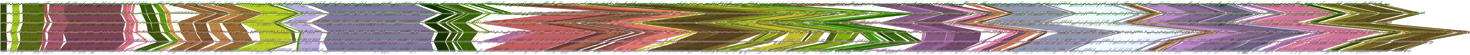
\includegraphics[width=1\textwidth]{images/collinear_zeae}  
  \end{center}
  When we compare two features (e.g. genes) between two or more genomes, there must be some basis for making the comparison \\
  That is, they have to be \textit{equivalent} in some way, such as:
  \begin{itemize}
    \item common evolutionary origin
    \item functional similarity
    \item a family-based relationship
  \end{itemize}
  It's common to define equivalence of genome features in terms of evolutionary relationship.
\end{frame}

% Gene features
\begin{frame}
  \frametitle{Evolutionary relationships\footnote{\tiny{Fitch (1970) \textit{Syst. Zool.} \textbf{19}:99-113 \href{http://dx.doi.org/10.2307/2412448}{doi:10.2307/2412448}}}}
  Equivalencies and relationships can be quite complex. \\
  We need precise terms to describe relationships between genome features. \\
  \begin{center}
    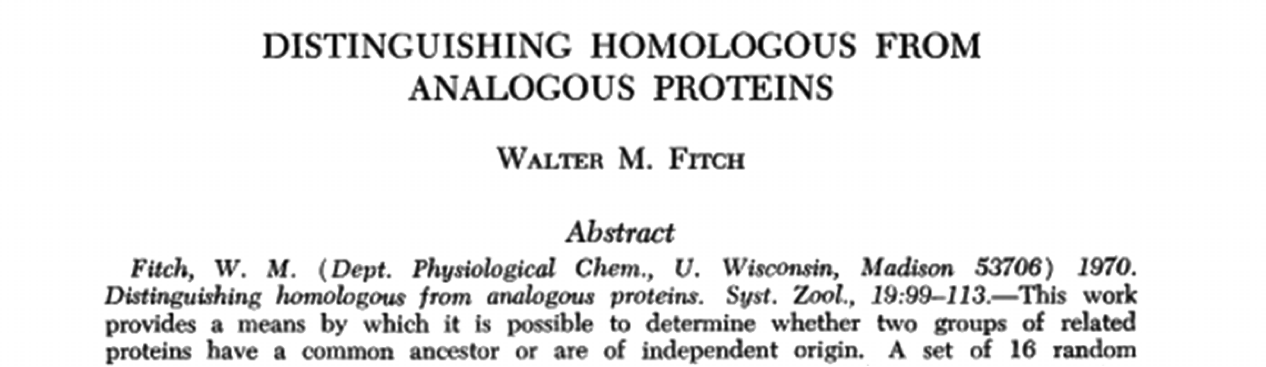
\includegraphics[width=1\textwidth]{images/fitch}  
  \end{center}  
  \begin{itemize}
    \item \textbf{analogy}: functional similarity
    \item \textbf{homology}: evolutionary common ancestor
  \end{itemize}    
\end{frame}



%%%
% SECTION: Homology, orthology and paralogy
\section{Homology, Orthology, Paralogy}
%% homology_orthology_paralogy.tex
%% Author: Leighton Pritchard
%% Copyright: James Hutton Institute
%% A brief description of the -logues
%% issues

% SUBSECTION: Genome Features
\subsection{What makes genome features equivalent?}

% ncRNA features
\begin{frame}
  \frametitle{Who let the -logues out?\footnote{\tiny{Fitch (2000) \textit{Trends Genet.} \textbf{16}:227-231 \href{http://dx.doi.org/10.1016/S0168-9525(00)02005-9}{doi:10.1016/S0168-9525(00)02005-9}}}}
    \begin{itemize}
      \item \textbf{homologues}: elements that are similar because they share a common ancestor. \textbf{There are NOT degrees of homology}
      \item \textbf{analogues}: elements that are (functionally?) similar, and this may be through common ancestry \textit{or} some other means, e.g. convergent evolution
      \item \textbf{orthologues}: homologues that diverged through speciation
      \item \textbf{prologues}: homologues that diverged through duplication within the same genome
    \end{itemize}
\end{frame}

% Regulatory features
\begin{frame}
  \frametitle{Who let the -logues out?}
  \begin{center}
    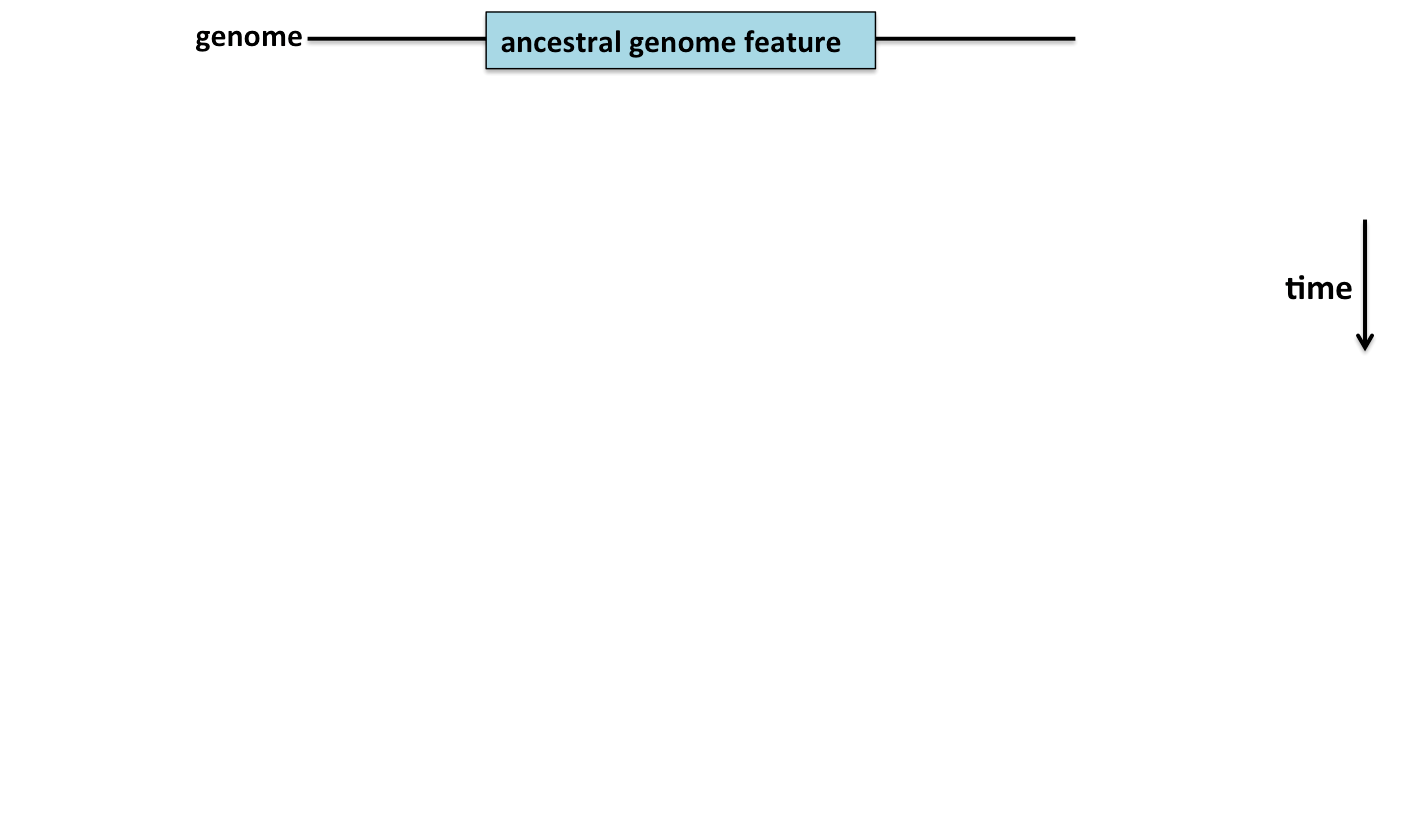
\includegraphics[width=1\textwidth]{images/logues1}  
  \end{center}  
\end{frame}

% Regulatory features
\begin{frame}
  \frametitle{Who let the -logues out?}
  \begin{center}
    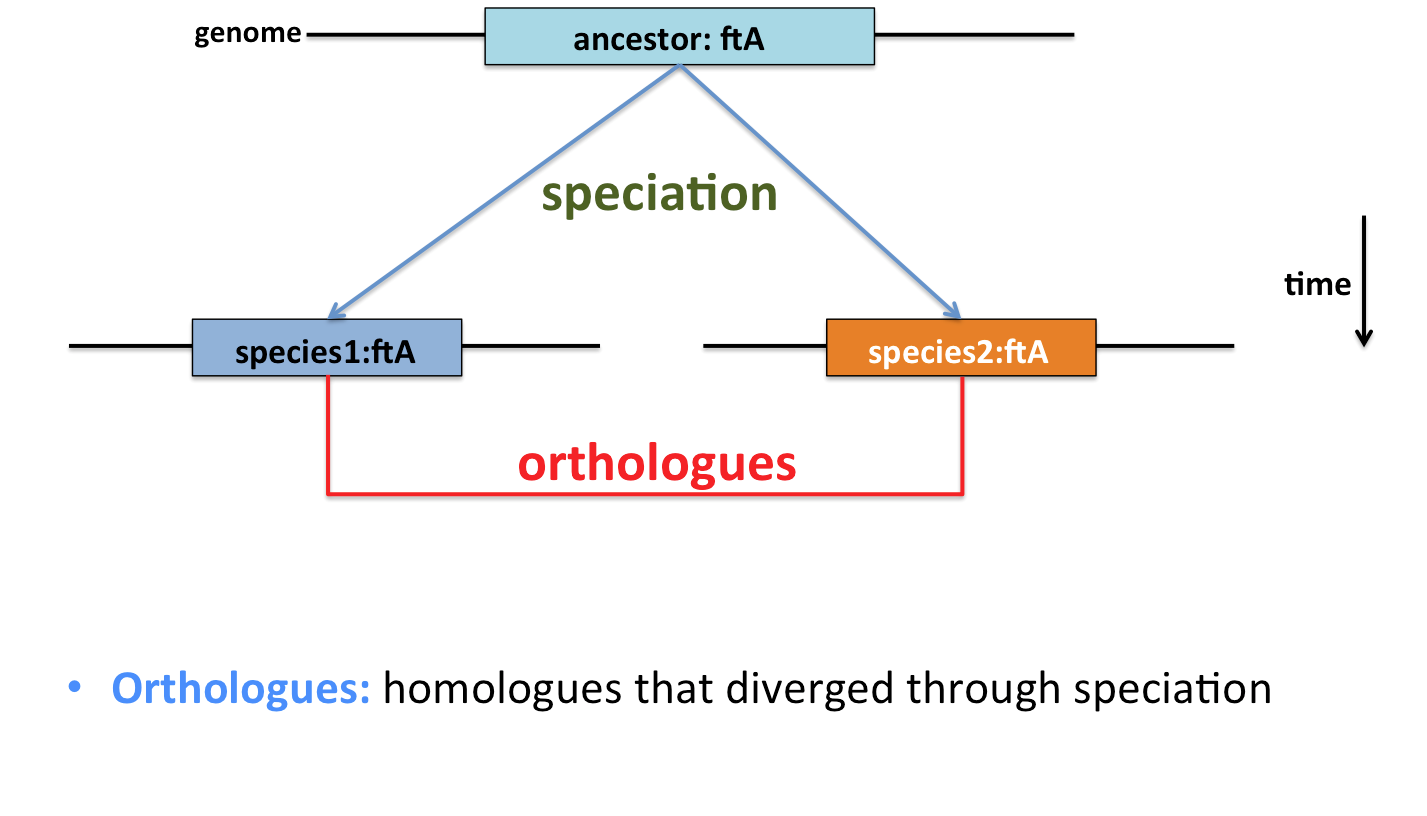
\includegraphics[width=1\textwidth]{images/logues2}  
  \end{center}  
\end{frame}

% Regulatory features
\begin{frame}
  \frametitle{Who let the -logues out?}
  \begin{center}
    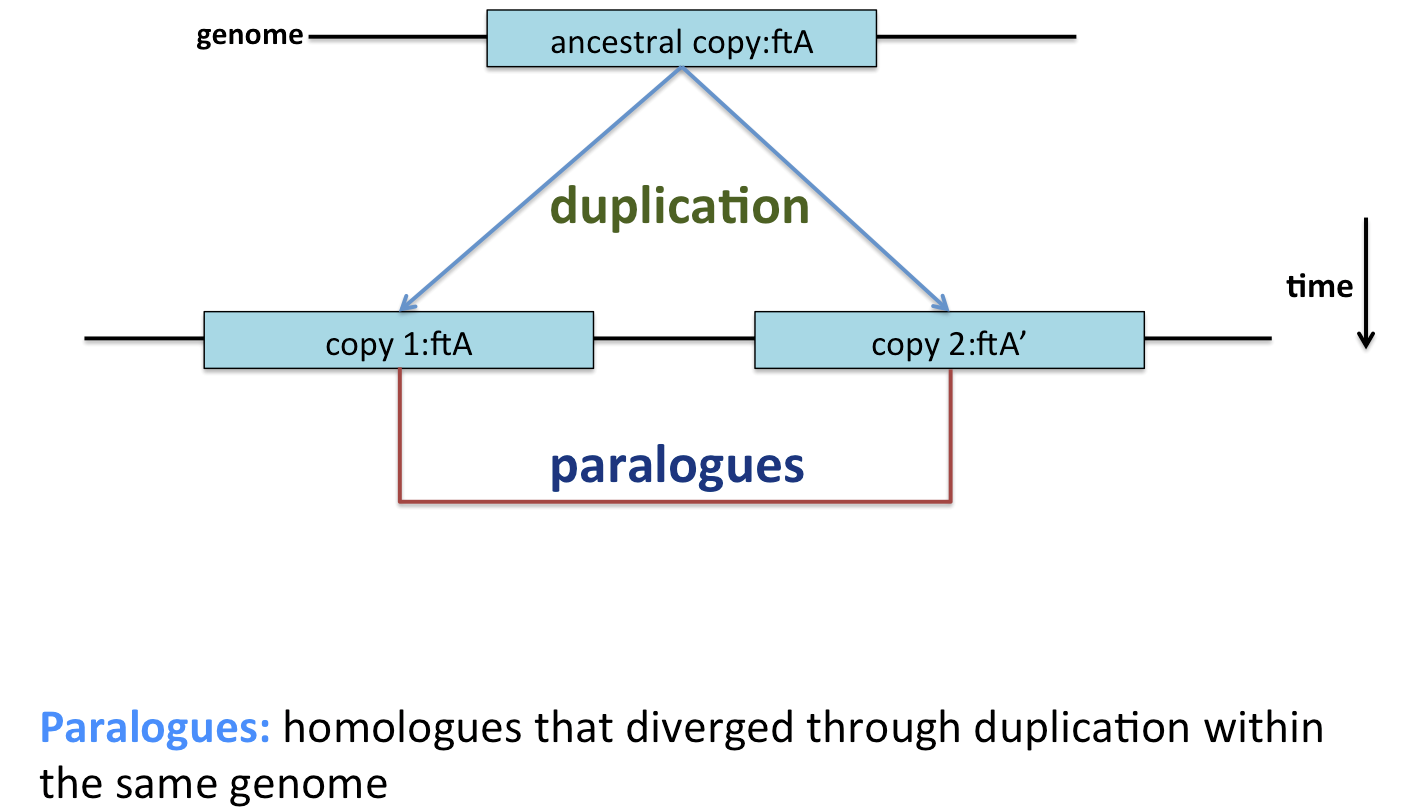
\includegraphics[width=1\textwidth]{images/logues3}  
  \end{center}  
\end{frame}

% Regulatory features
\begin{frame}
  \frametitle{Who let the -logues out?}
  \begin{center}
    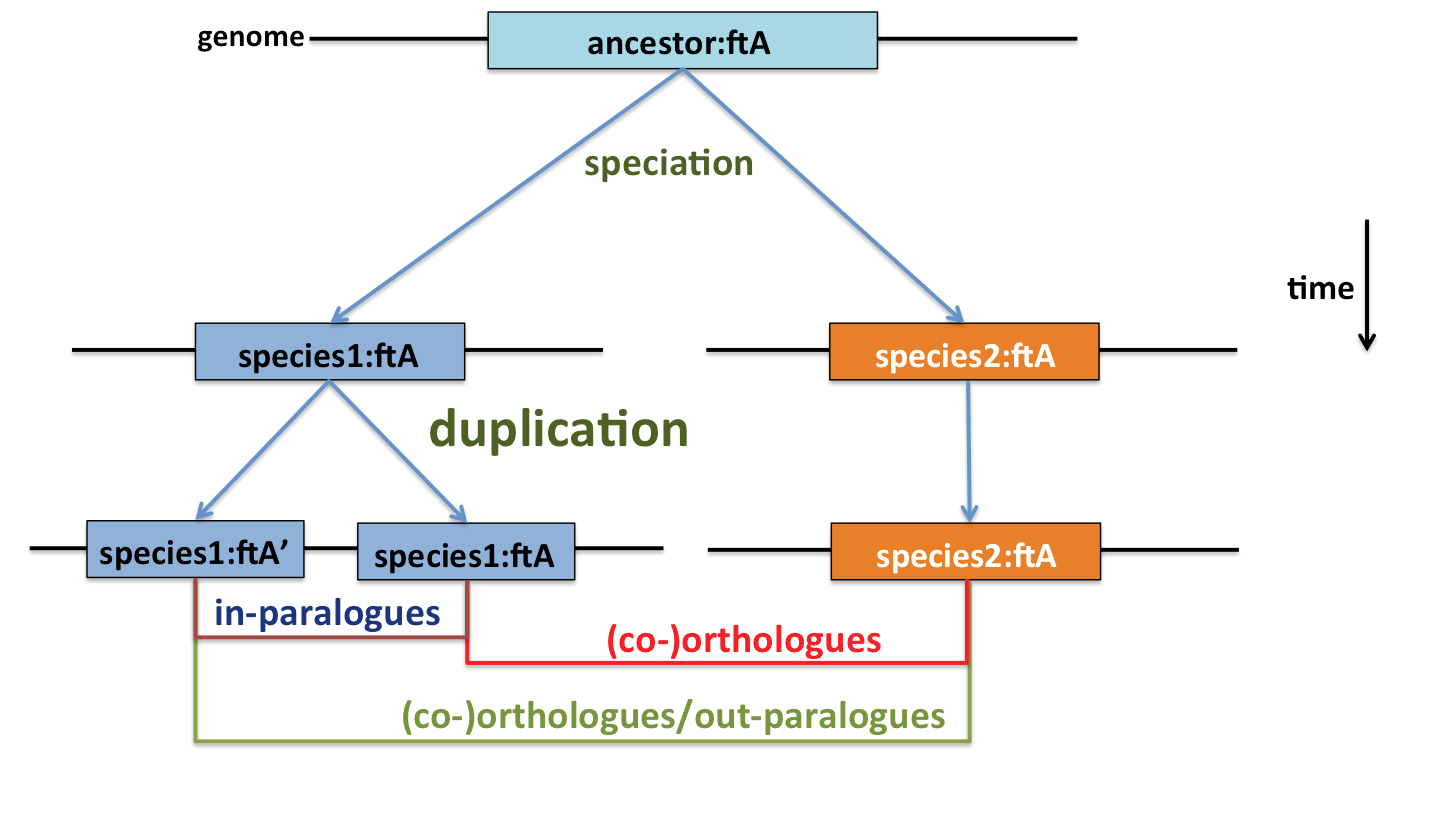
\includegraphics[width=1\textwidth]{images/logues4}  
  \end{center}  
\end{frame}

% Regulatory features
\begin{frame}
  \frametitle{Who let the -logues out?}
  \begin{center}
    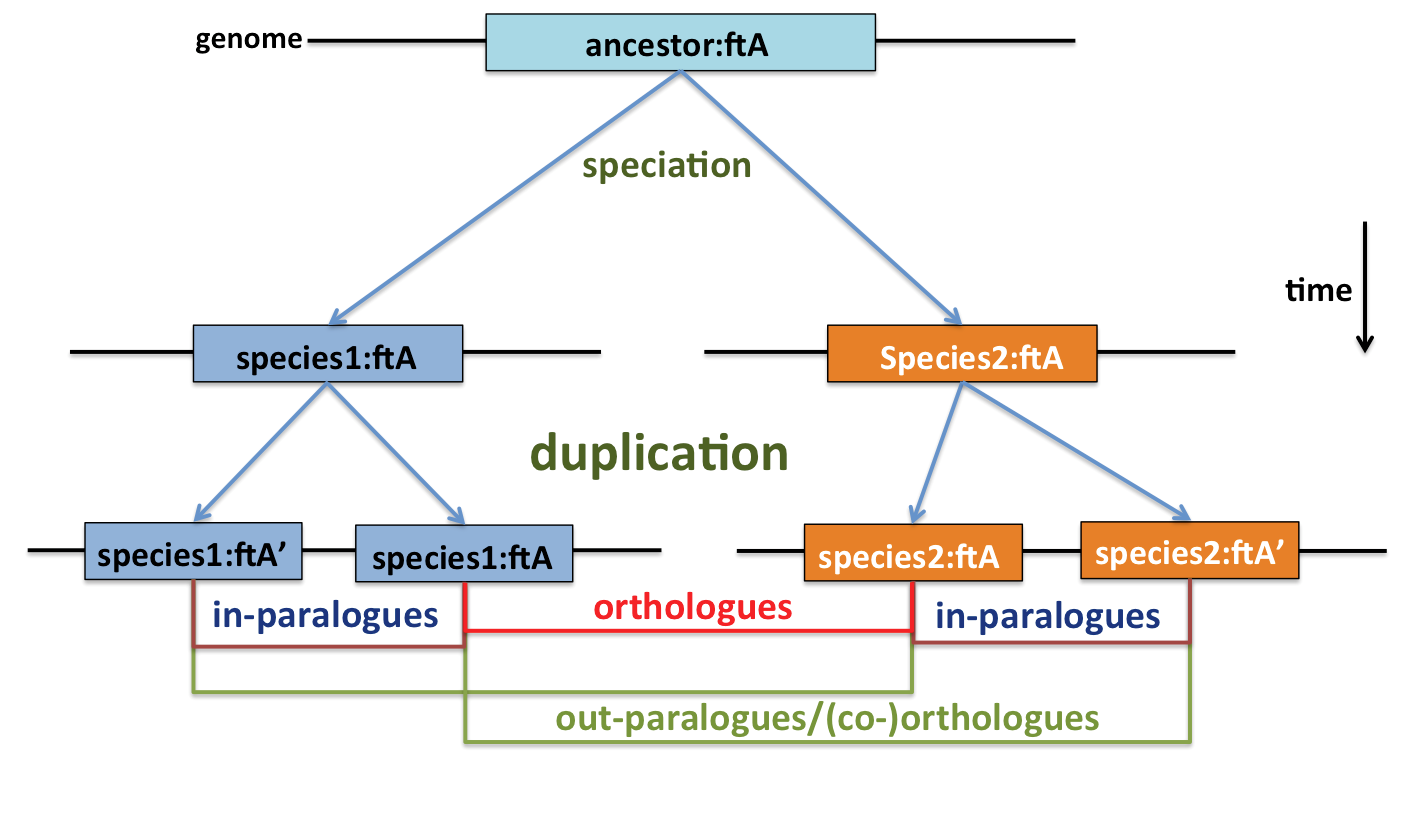
\includegraphics[width=1\textwidth]{images/logues5}  
  \end{center}  
\end{frame}

% Principles of feature prediction
\begin{frame}
  \frametitle{ITYFIALMCTT\footnote{\tiny{Kristensen \textit{et al}. (2011) \textit{Brief. Bioinf.} \textbf{12}:379-391 \href{http://dx.doi.org/10.1093/bib/bbr030}{doi:10.1093/bib/bbr030}}}}
  But it's a little more complicated than that. \\
  Biology is not well-behaved.
  \begin{itemize}
    \item Gene loss
    \item Homologues may diverge so widely that they can be hard to recognise
    \item Reconstructed evolutionary trees may not be robust inferences of speciation (or relevant to it, in prokaryotes)
    \item There is no record of history - we can only make inferences
  \end{itemize}
  \textbf{All classifications of orthology/paralogy are inferences!}
\end{frame}

% Principles of feature prediction
\begin{frame}
  \frametitle{ITYFIALMCTT\footnote{\tiny{Kristensen \textit{et al}. (2011) \textit{Brief. Bioinf.} \textbf{12}:379-391 \href{http://dx.doi.org/10.1093/bib/bbr030}{doi:10.1093/bib/bbr030}}}}
  \begin{center}
    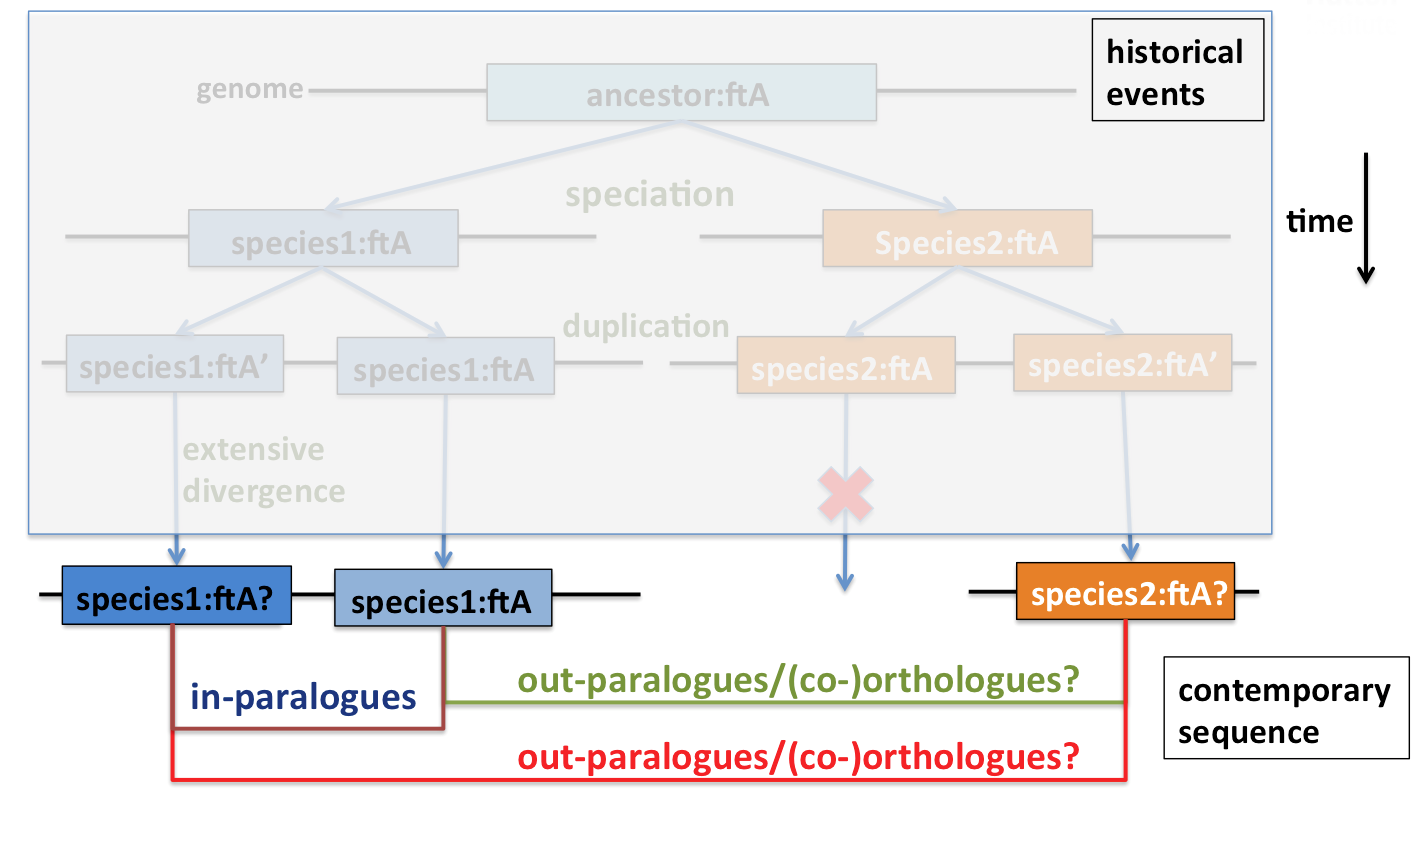
\includegraphics[width=1\textwidth]{images/logues6}  
  \end{center} 
  \textbf{All classifications of orthology/paralogy are inferences!}
\end{frame}

\begin{frame}
  \frametitle{Ensembl Compara\footnote{\tiny{Vilella \textit{et al}. (2009) \textit{Genome Res.} \textbf{19}:327-335 \href{http://dx.doi.org/10.1101/gr.073585.107}{doi:10.1101/gr.073585.107}}}}
  Some tools/databases, e.g. \href{http://www.ensembl.org/info/genome/compara/index.html}{Ensembl Compara}, use slightly different definitions
  \begin{center}
    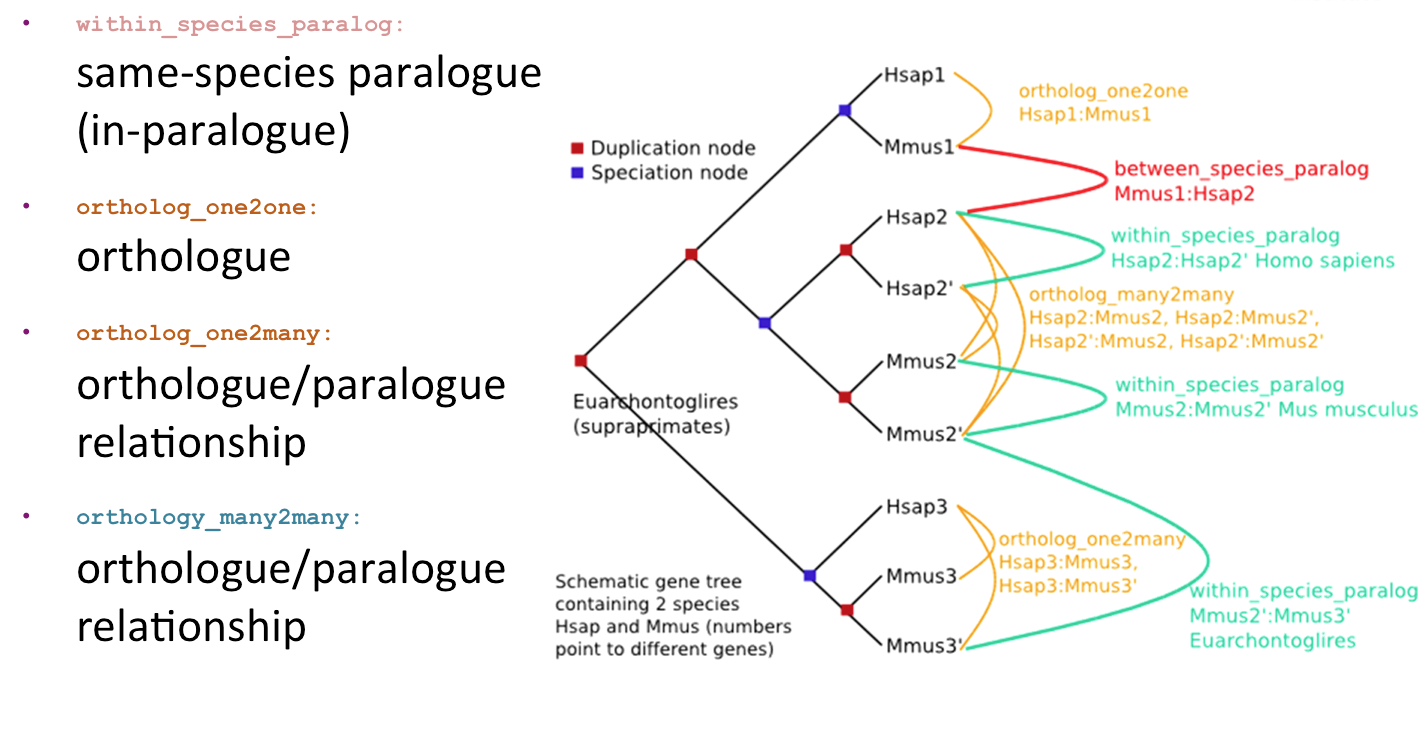
\includegraphics[width=1\textwidth]{images/logues7}  
  \end{center} 
\end{frame}
%% orthologue_prediction.tex
%% Author: Leighton Pritchard
%% Copyright: James Hutton Institute
%% A brief introduction to orthologues, and their prediction

% SUBSECTION: Why orthologues?
\subsection{What's so important about orthologues?}

% Why focus on orthologues
\begin{frame}
  \frametitle{Why focus on orthologues?}
  Formalise the idea of \textit{corresponding genes} in different organisms. \\
  Orthologues serve two purposes:
  \begin{itemize}
    \item \textbf{Evolutionary equivalence}
    \item \textbf{Functional equivalence} (``The Ortholog Conjecture''\footnote{\tiny{Chen and Zhang (2012) \textit{PLoS Comp. Biol.} \textbf{8}:e1002784 \href{http://dx.doi.org/10.1371/journal.pcbi.1002784}{doi:10.1371/journal.pcbi.1002784}}})
  \end{itemize}
  Applications in comparative genomics, functional genomics and phylogenetics.\footnote{\tiny{Dessimoz (2011) \textit{Brief. Bioinf.} \textbf{12}:375-376 \href{http://dx.doi.org/10.1093/bib/bbr057}{doi:10.1093/bib/bbr057}}} \\
  Over 30 databases attempt to describe orthologous relationships (\href{http://questfororthologs.org/orthology_databases
}{http://questfororthologs.org/orthology\_databases}\footnote{\tiny{Altenhoff and Dessimoz (2009) \textit{PLoS Comp. Biol.} \textbf{5}:e1000262 \href{http://dx.doi.org/10.1371/journal.pcbi.1000262}{doi:10.1371/journal.pcbi.1000262}}})
\end{frame}

% Orthologue-finding methods
\begin{frame}
  \frametitle{Finding orthologues}
      Multiple methods and databases%
\footnote{\tiny{Kristensen \textit{et al}. (2011) \textit{Brief. Bioinf.} \textbf{12}:379-391 \href{http://dx.doi.org/10.1093/bib/bbr030}{doi:10.1093/bib/bbr030}}}$^,$%
\footnote{\tiny{Trachana \textit{et al}. (2011) \textit{Bioessays} \textbf{33}:769-780 \href{http://dx.doi.org/10.1002/bies.201100062}{doi:10.1002/bies.201100062}}}$^,$%
\footnote{\tiny{Salichos and Rokas (2011) \textit{PLoS One} \textbf{6}:e18755 \href{http://dx.doi.org/10.1371/journal.pone.0018755.g006}{doi:10.1371/journal.pone.0018755.g006}}}
  \begin{columns}[T]    \begin{column}{6cm}
      \begin{itemize}
        \item \textbf{Pairwise genome}
        \begin{itemize}
          \item \href{http://armchairbiology.blogspot.co.uk/2012/07/on-reciprocal-best-blast-hits.html}{RBBH} (aka BBH, RBH), \href{http://link.springer.com/protocol/10.1007/978-1-59745-515-2_7}{RSD}, \href{http://inparanoid.sbc.su.se/cgi-bin/index.cgi}{InParanoid}, \href{http://roundup.hms.harvard.edu/}{RoundUp}
        \end{itemize}
        \item \textbf{Multi-genome}
        \begin{itemize}
          \item Graph-based: \href{http://www.ncbi.nlm.nih.gov/COG/}{COG}, \href{http://eggnog.embl.de/}{eggNOG}, \href{http://cegg.unige.ch/orthodb7}{OrthoDB}, \href{http://orthomcl.org/orthomcl/}{OrthoMCL}, \href{http://omabrowser.org/cgi-bin/gateway.pl}{OMA}, \href{http://multiparanoid.sbc.su.se/}{MultiParanoid}
          \item Tree-based: \href{http://www.treefam.org/}{TreeFam}, \href{http://www.ensembl.org/info/genome/compara/index.html}{Ensembl Compara}, \href{http://phylomedb.org/}{PhylomeDB}, \href{https://trac.nbic.nl/loft/}{LOFT}
        \end{itemize}
      \end{itemize}
    \end{column}
    \begin{column}{4cm}
      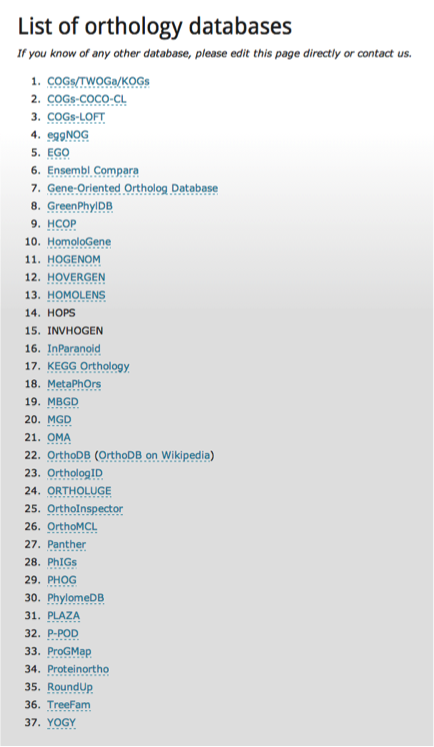
\includegraphics[height=0.6\textheight]{images/orthology_databases}      
    \end{column}
  \end{columns}
\end{frame}


%% evaluating_orthologue_prediction.tex
%% Author: Leighton Pritchard
%% Copyright: James Hutton Institute
%% A brief introduction to orthologues, and evaluation of their prediction

% SUBSECTION: Why orthologues?
\subsection{Evaluating orthologue prediction}

% Which methods work best
\begin{frame}
  \frametitle{Which prediction methods work best?}
  Taking advantage of prokaryotic operon structure: \textbf{if the outer pair of a syntenic triplet of genes are orthologous, the middle gene is also likely to be orthologous}.\footnote{\tiny{Wolf and Koonin (2012) \textit{Genome Biol. Evil.} \textbf{4}:1286-1294 \href{http://dx.doi.org/10.1093/gbe/evs100}{doi:10.1093/gbe/evs100}}}\\
  Specifically testing reciprocal best hits (RBH).
  \begin{center}
      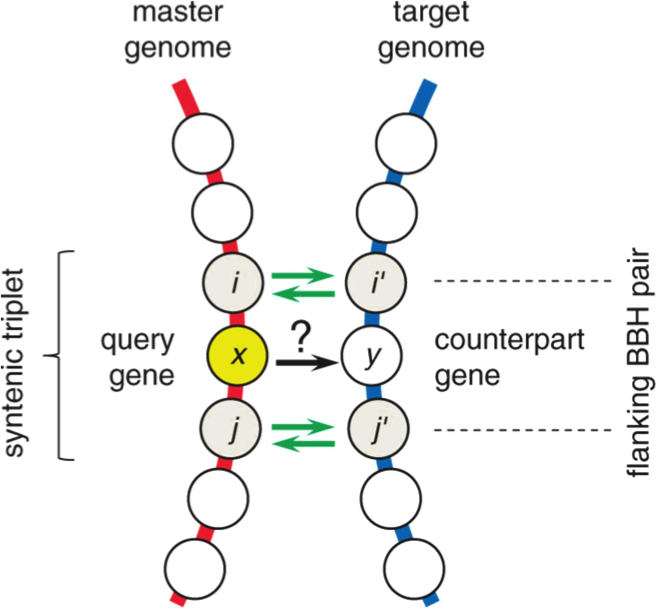
\includegraphics[height=0.45\textheight]{images/syntenic_triplet} 
  \end{center}
\end{frame}

% Which methods work best
\begin{frame}
  \frametitle{Which prediction methods work best?}
  \begin{itemize}
    \item Tested on 573 prokaryotic genomes
    \item 88-99\% of RBH found in syntenic triplets
    \item Overwhelming majority of middle genes are RBH
  \end{itemize}
  \textbf{RBH reliably finds orthologues.}\footnote{\tiny{Wolf and Koonin (2012) \textit{Genome Biol. Evil.} \textbf{4}:1286-1294 \href{http://dx.doi.org/10.1093/gbe/evs100}{doi:10.1093/gbe/evs100}}}
  \begin{center}
      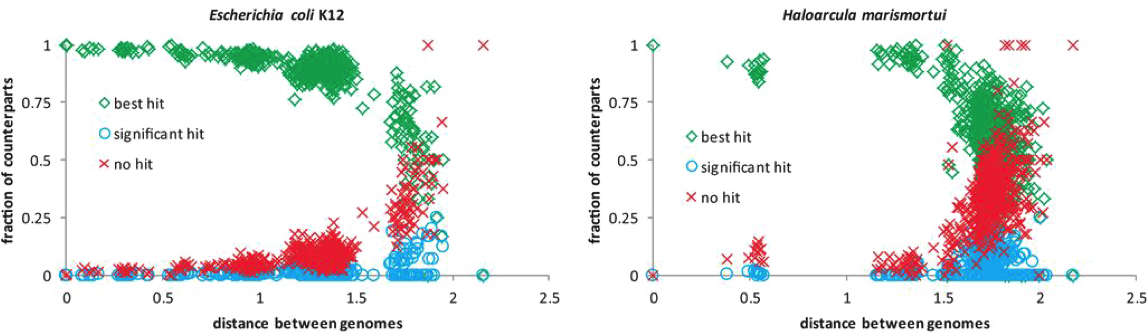
\includegraphics[width=1\textwidth]{images/syntenic_triplet_results} 
  \end{center}
\end{frame}

% Which methods work best
\begin{frame}
  \frametitle{Which prediction methods work best?}
  Four methods tested against 2,723 curated orthologues from six \textit{Saccharomycetes}
  \begin{itemize}
    \item RBBH (and cRBH); RSD (and cRSD); MultiParanoid; OrthoMCL
    \item Rated by statistical performance metrics: sensitivity, specificity, accuracy, FDR
  \end{itemize}
  \textbf{cRBH most accurate and specific, with lowest FDR.}\footnote{\tiny{Salichos and Rokas (2011) \textit{PLoS One} \textbf{6}:e18755 \href{http://dx.doi.org/10.1371/journal.pone.0018755.g006}{doi:10.1371/journal.pone.0018755.g006}}}
  \begin{center}
      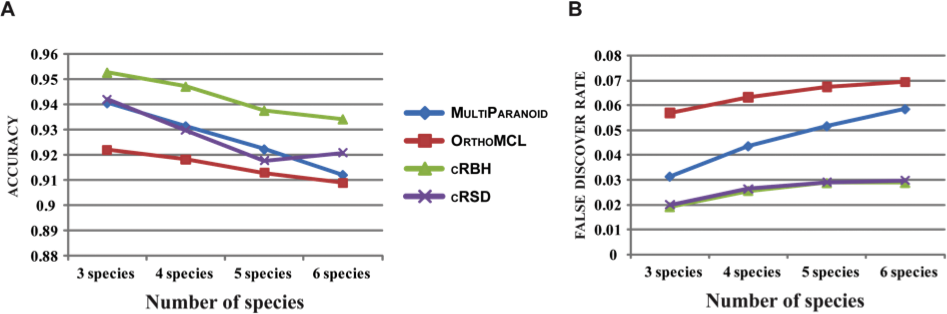
\includegraphics[height=0.25\textheight]{images/salichos_results1} 
      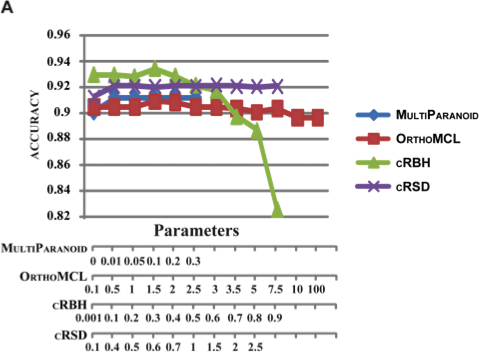
\includegraphics[height=0.25\textheight]{images/salichos_results2}      
  \end{center}
\end{frame}

% Which methods work best
\begin{frame}
  \frametitle{Which prediction methods work best?}
  Testing on literature-based benchmarks for grouping by function and correct branching of phylogeny.\footnote{\tiny{Altenhoff and Dessimoz (2009) \textit{PLoS Comp. Biol.} \textbf{5}:e1000262 \href{http://dx.doi.org/10.1371/journal.pcbi.1000262}{doi:10.1371/journal.pcbi.1000262}}}
  \begin{center}
      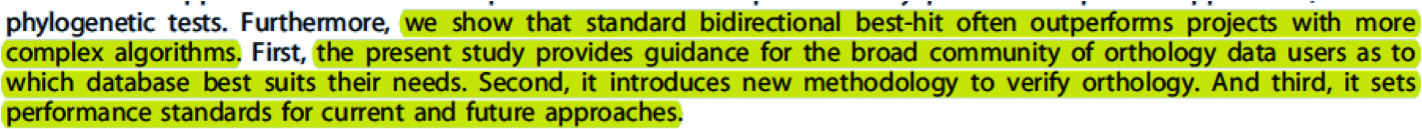
\includegraphics[width=1\textwidth]{images/altenhoff1} \\
      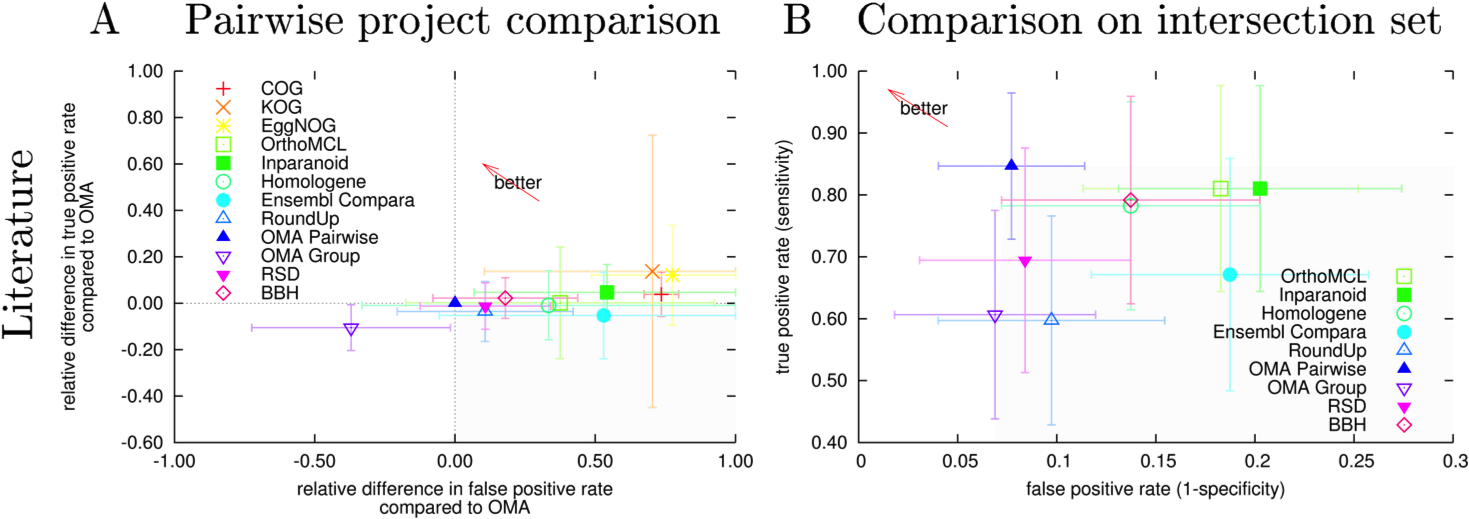
\includegraphics[width=1\textwidth]{images/altenhoff2}      
  \end{center}
\end{frame}

% Which methods work best
\begin{frame}
  \frametitle{Which prediction methods work best?}
  \begin{itemize}
    \item Performance varies by choice of method, and interpretation of ``orthology''
    \item Biggest influence is genome annotation quality
    \item Relative performance varies with choice of benchmark
    \item \textbf{(clustering) RBH outperforms more complex algorithms under many circumstances}
  \end{itemize}
\end{frame}

% Which methods work best
\begin{frame}
  \frametitle{What is this magic RBH method?}
  \begin{center}
      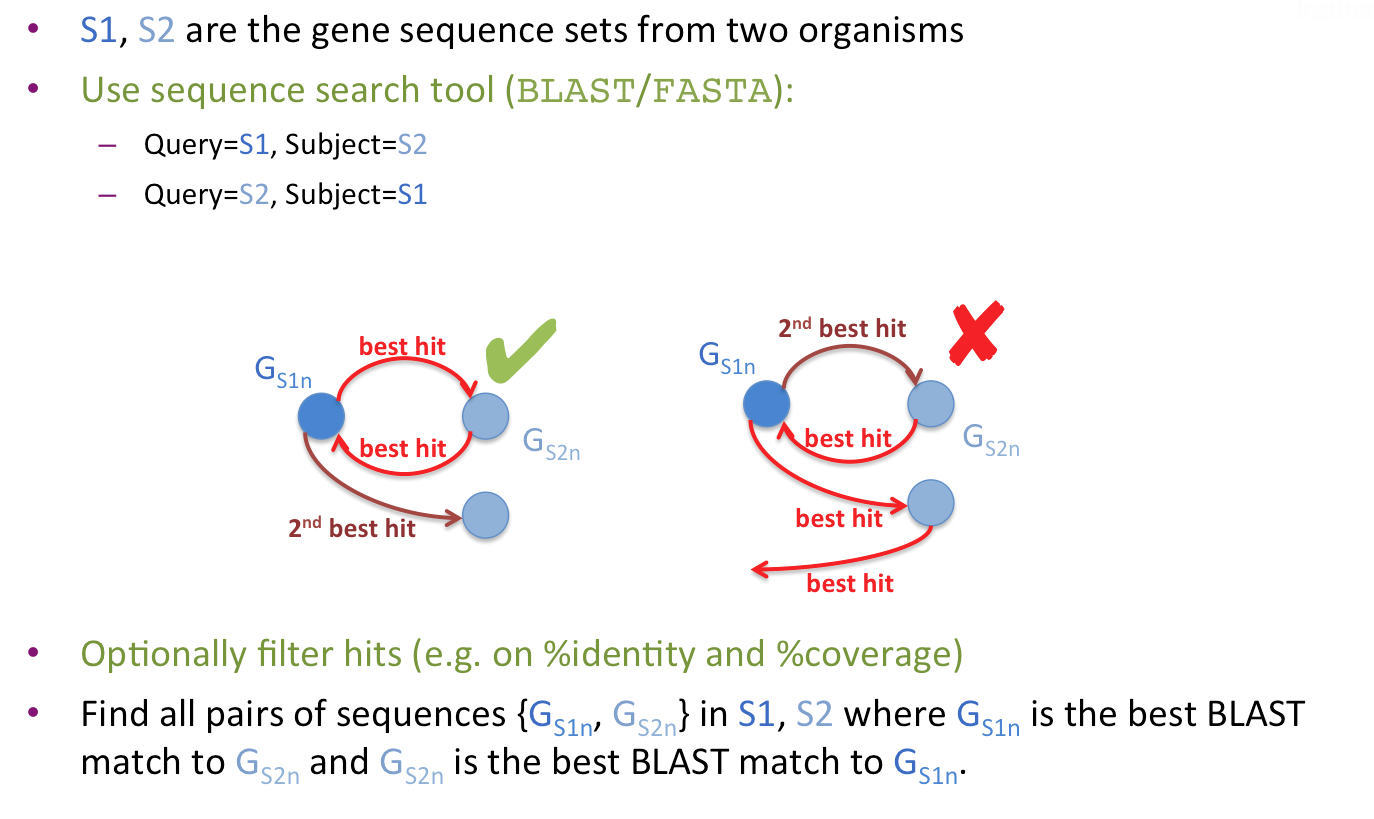
\includegraphics[width=1\textwidth]{images/rbbh}      
  \end{center}
\end{frame}
%% using_orthologue_prediction.tex
%% Author: Leighton Pritchard
%% Copyright: James Hutton Institute
%% A brief introduction to orthologues, and evaluation of their prediction

% SUBSECTION: Why orthologues?
\subsection{Using orthologue predictions}

% Which methods work best
\begin{frame}
  \frametitle{Functional adaptation in \textit{Pba}\footnote{\tiny{Toth \textit{et al}. (2006) \textit{Ann. Rev. Phytopath.} \textbf{44}:305-336 \href{http://dx.doi.org/10.1146/annurev.phyto.44.070505.143444}{doi:10.1146/annurev.phyto.44.070505.143444}}}}
  \begin{center}
      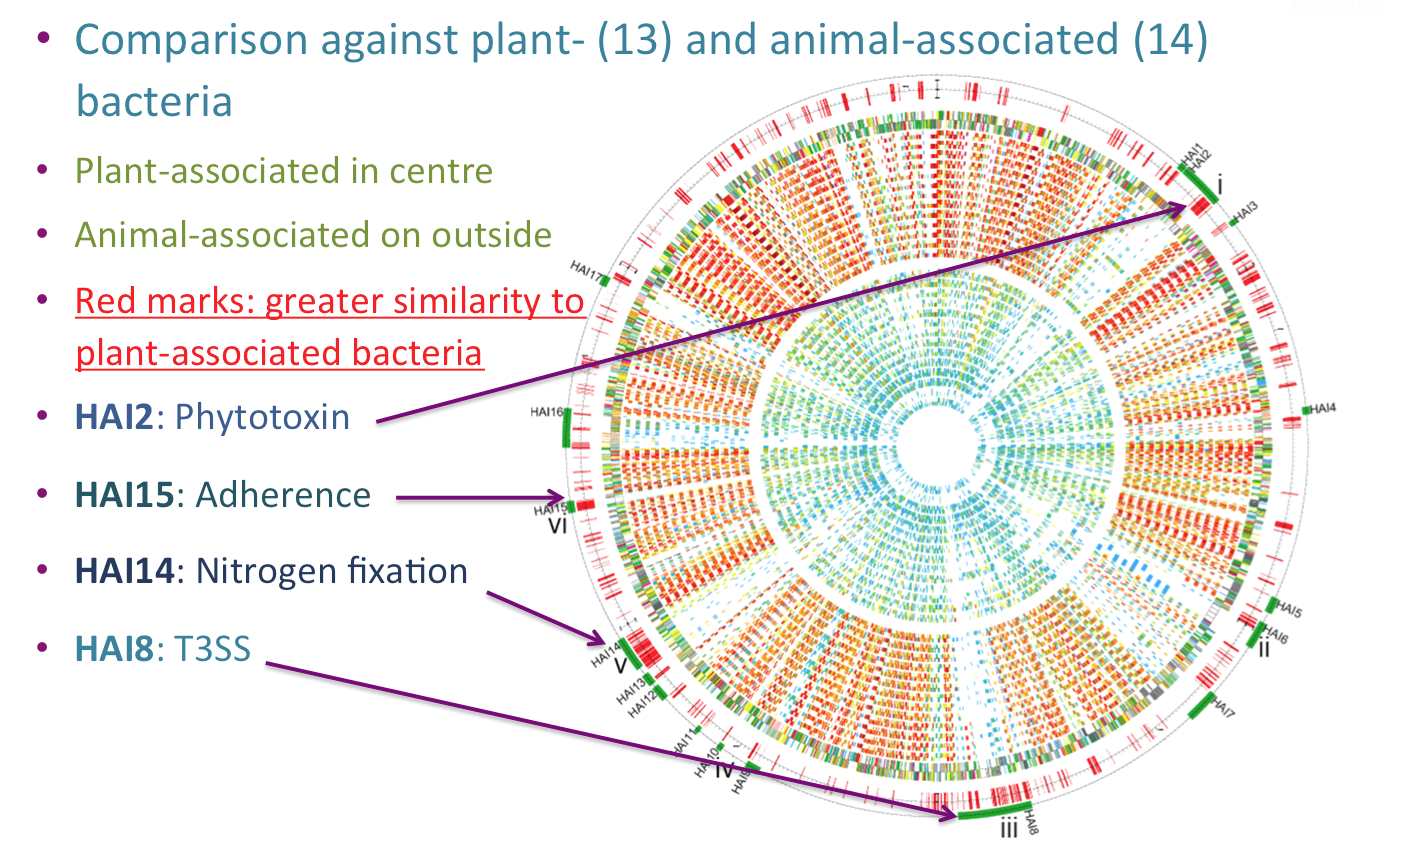
\includegraphics[width=1\textwidth]{images/pba_lgt} 
  \end{center}
\end{frame}

% Which methods work best
\begin{frame}
  \frametitle{Functional adaptation in \textit{Pba}\footnote{\tiny{Toth \textit{et al}. (2006) \textit{Ann. Rev. Phytopath.} \textbf{44}:305-336 \href{http://dx.doi.org/10.1146/annurev.phyto.44.070505.143444}{doi:10.1146/annurev.phyto.44.070505.143444}}}}
  \begin{center}
      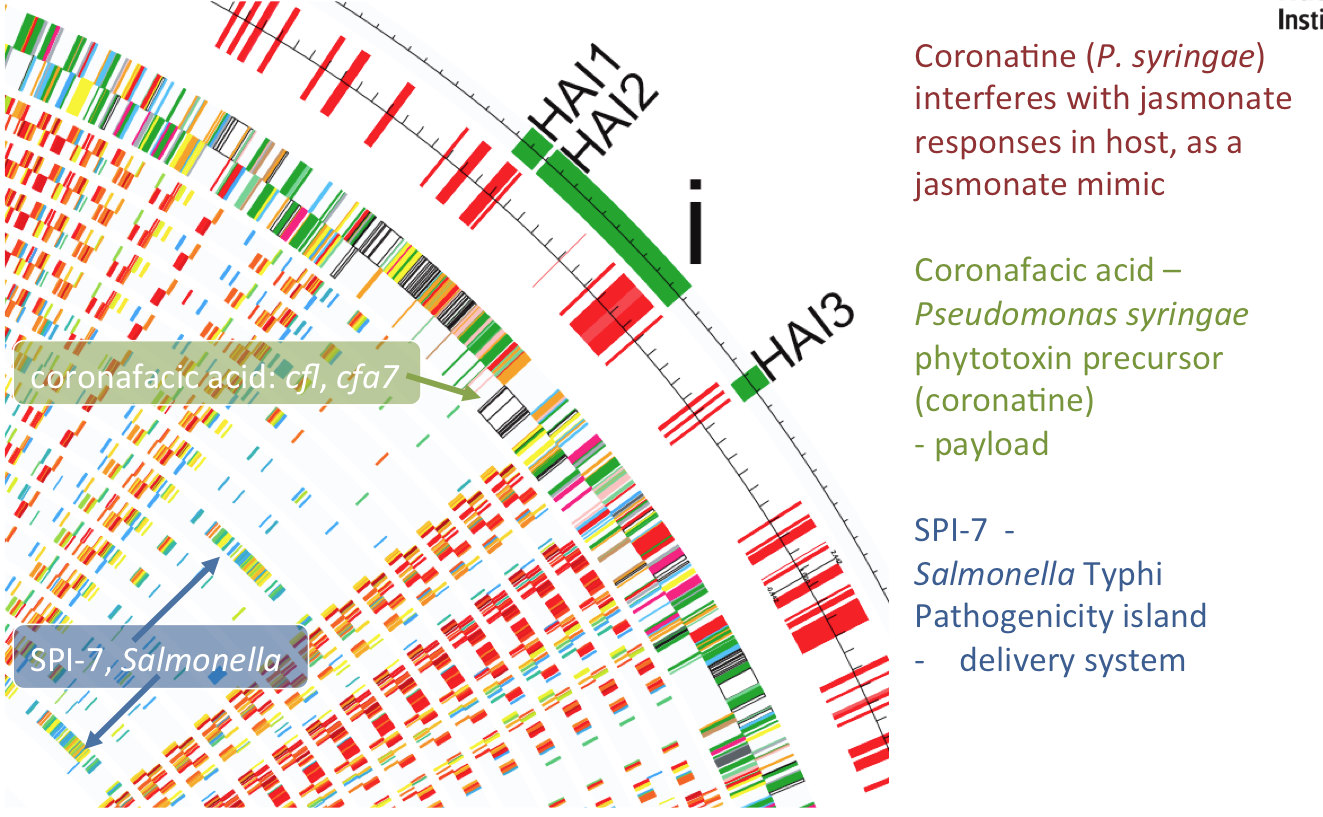
\includegraphics[width=1\textwidth]{images/pba_coronatine} 
  \end{center}
\end{frame}

% SUBSECTION: Core and pangenomes
\subsection{Core and Pan-genomes}

\begin{frame}
  \frametitle{Functional adaptation in \textit{Pba}\footnote{\tiny{Toth \textit{et al}. (2006) \textit{Ann. Rev. Phytopath.} \textbf{44}:305-336 \href{http://dx.doi.org/10.1146/annurev.phyto.44.070505.143444}{doi:10.1146/annurev.phyto.44.070505.143444}}}}
  \begin{center}
      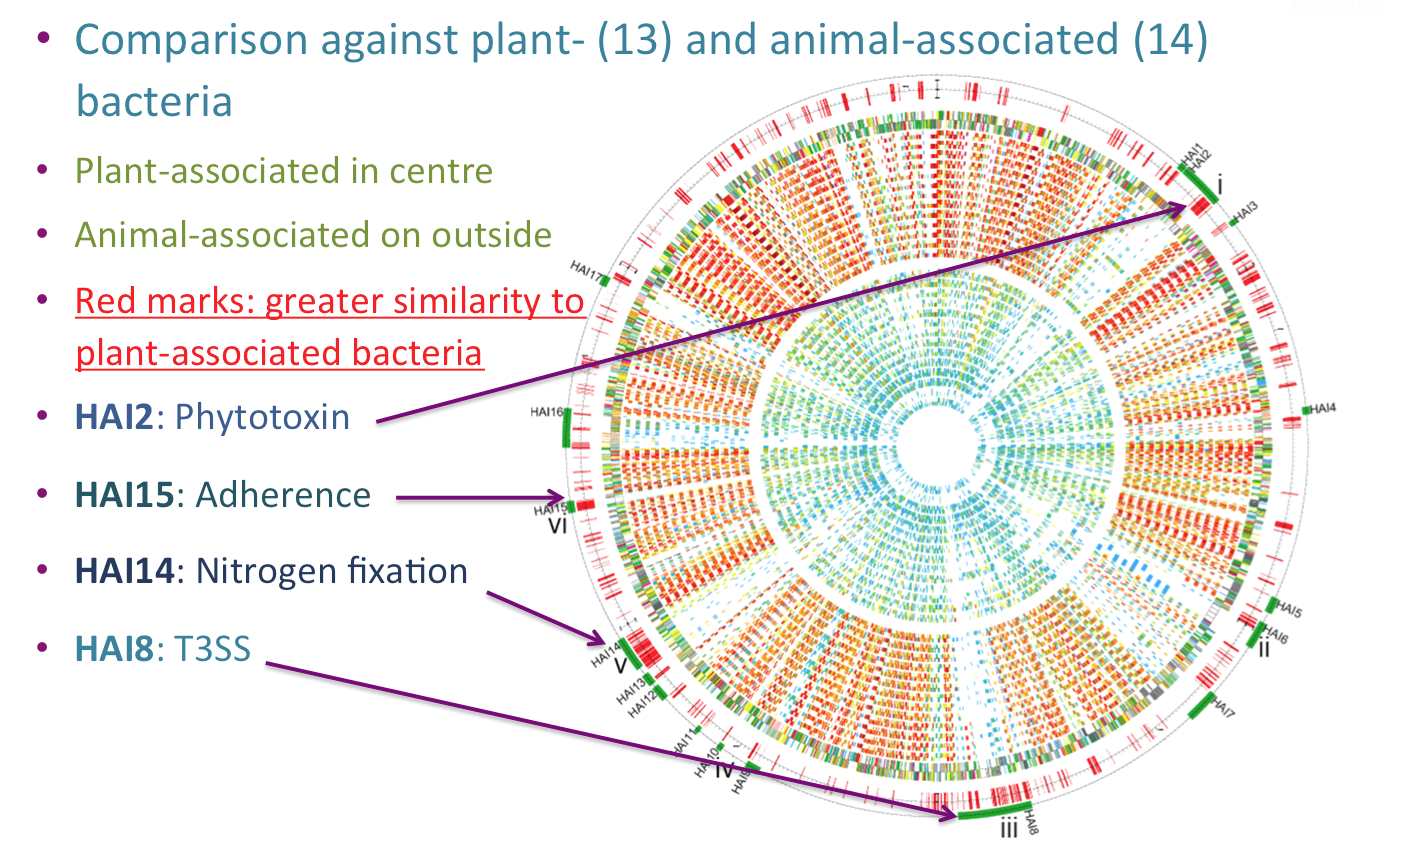
\includegraphics[width=1\textwidth]{images/pba_lgt} 
  \end{center}
\end{frame}



%%%
% SECTION: Conclusions
\section{Conclusions}
%% didnt_get_to.tex
%% Author: Leighton Pritchard
%% Copyright: James Hutton Institute
%% A brief introduction to orthologues, and evaluation of their prediction

% Things I didn't get to?
\subsection{Things I Didn't Get To}

% A set of topics I didn't get to cover, but with links
\begin{frame}
  \frametitle{Things I didn't get to}
  \begin{center}
      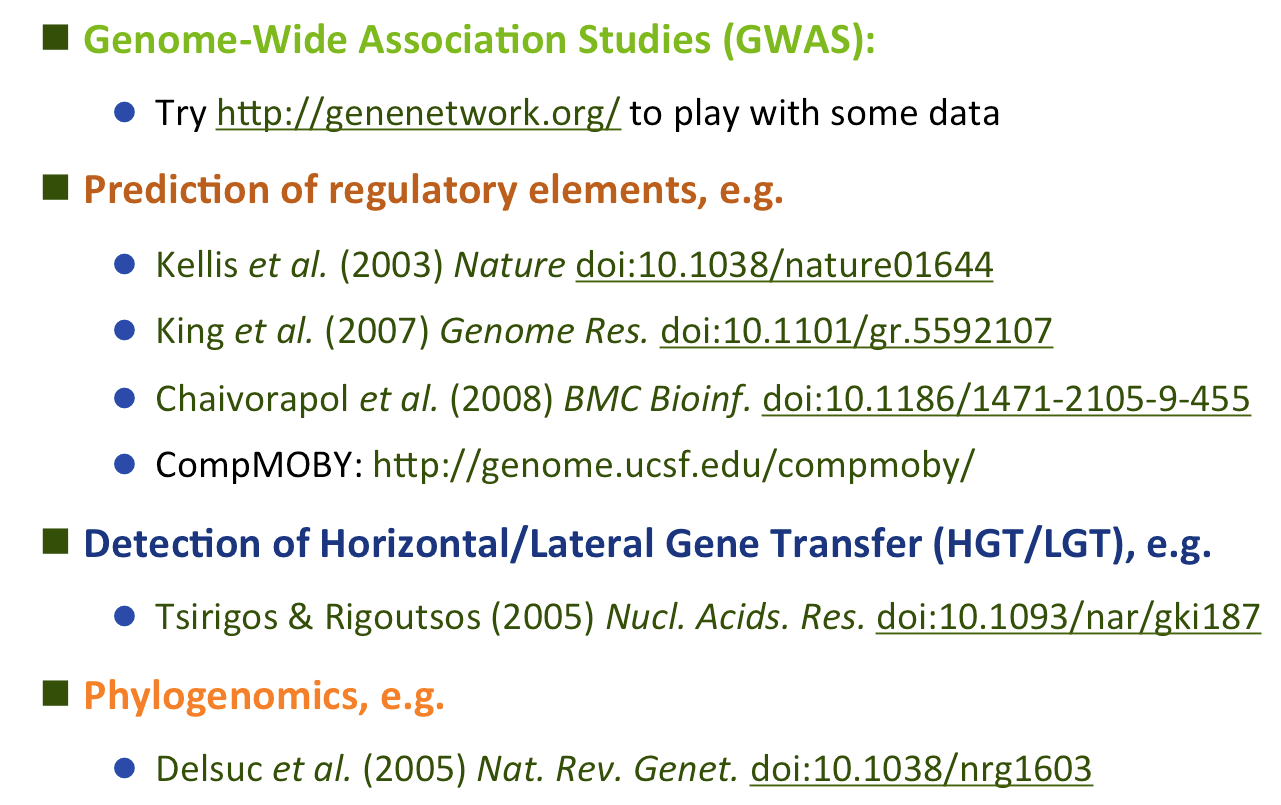
\includegraphics[width=1\textwidth]{images/didnt_get_to} 
  \end{center}
\end{frame}

%% conclusions.tex
%% Author: Leighton Pritchard
%% Copyright: James Hutton Institute
%% A brief introduction to orthologues, and evaluation of their prediction

% Conclusions
\subsection{Things I Didn't Get To}

% Which methods work best
\begin{frame}
  \frametitle{Things I didn't get to}
  \begin{center}
      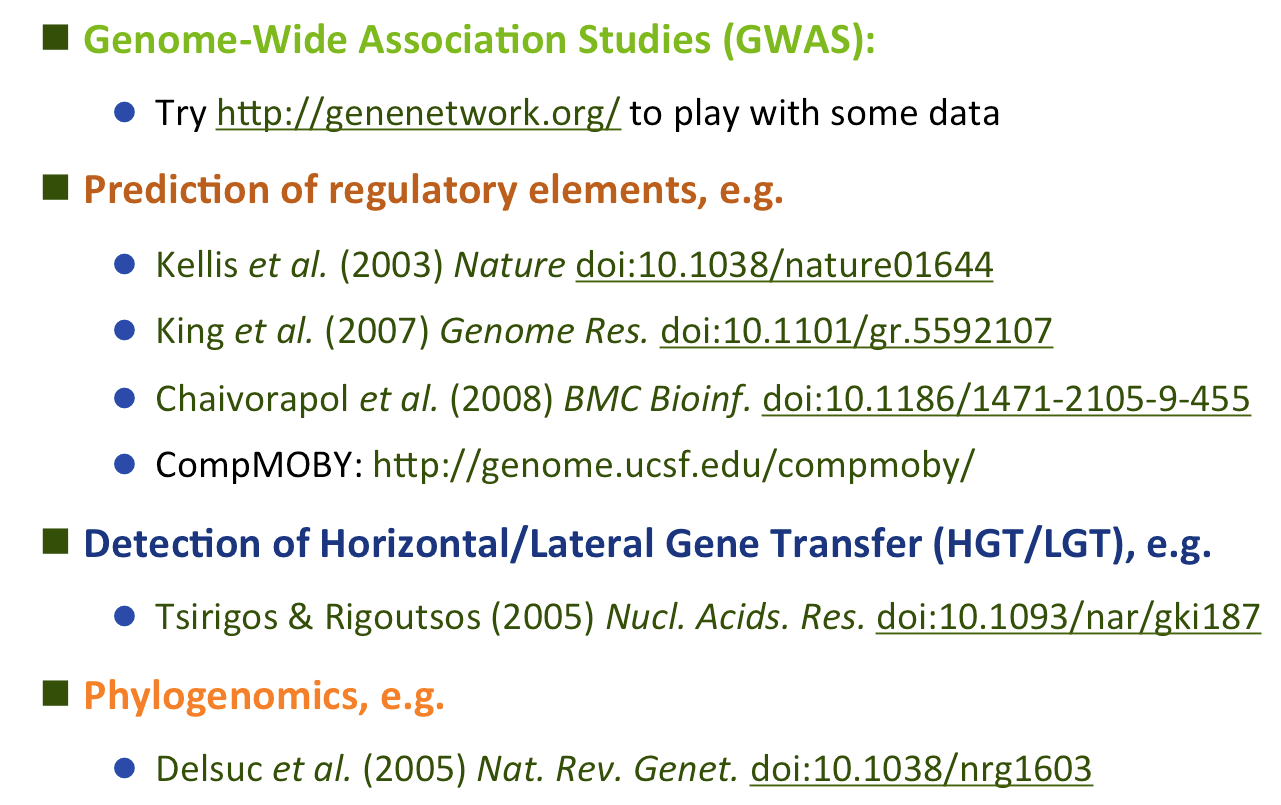
\includegraphics[width=1\textwidth]{images/didnt_get_to} 
  \end{center}
\end{frame}

% Conclusions
\subsection{Conclusions}

% Which methods work best
\begin{frame}
  \frametitle{Conclusions}
  \begin{center}
      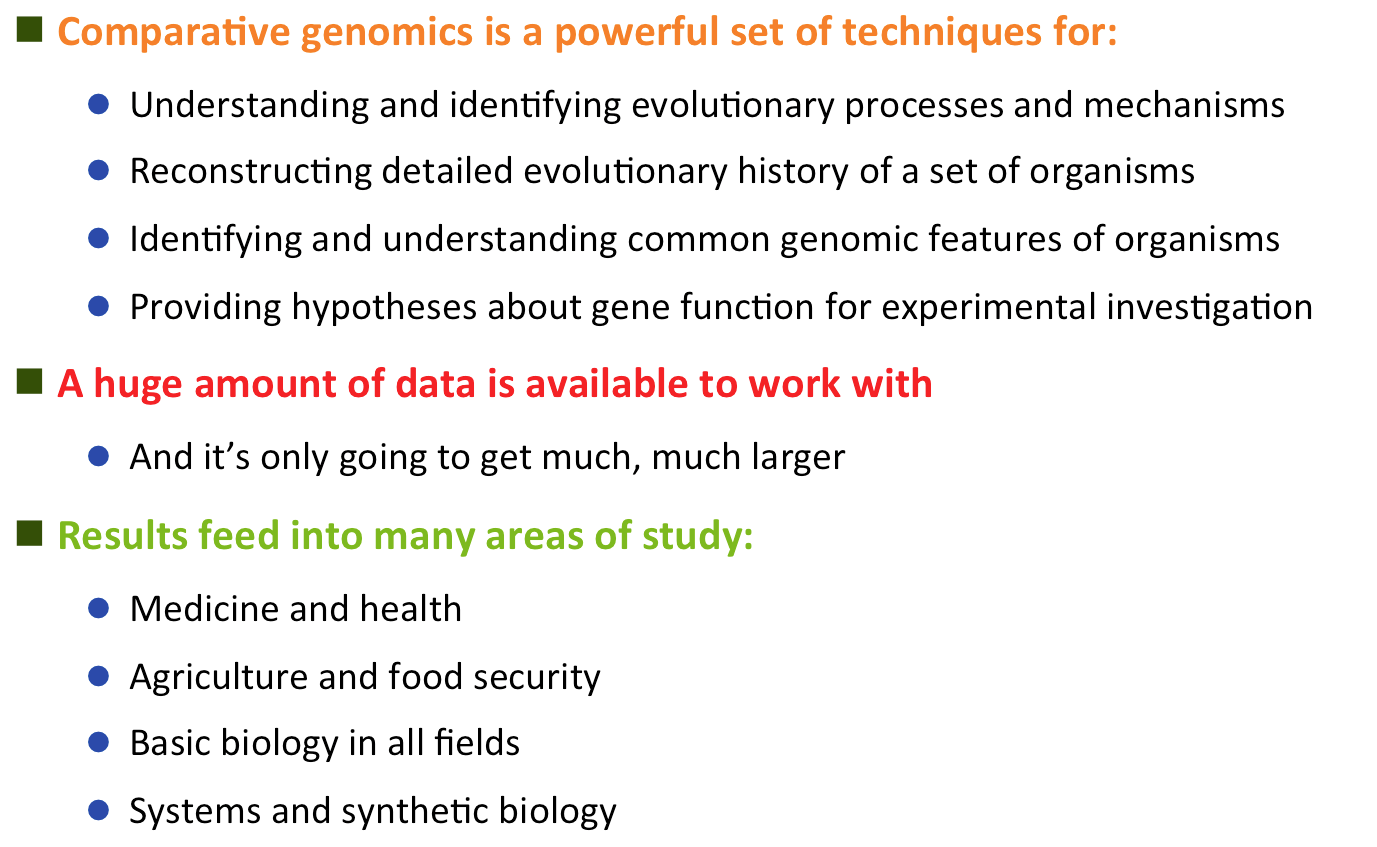
\includegraphics[width=1\textwidth]{images/conclusions1} 
  \end{center}
\end{frame}

% Which methods work best
\begin{frame}
  \frametitle{Conclusions}
  \begin{center}
      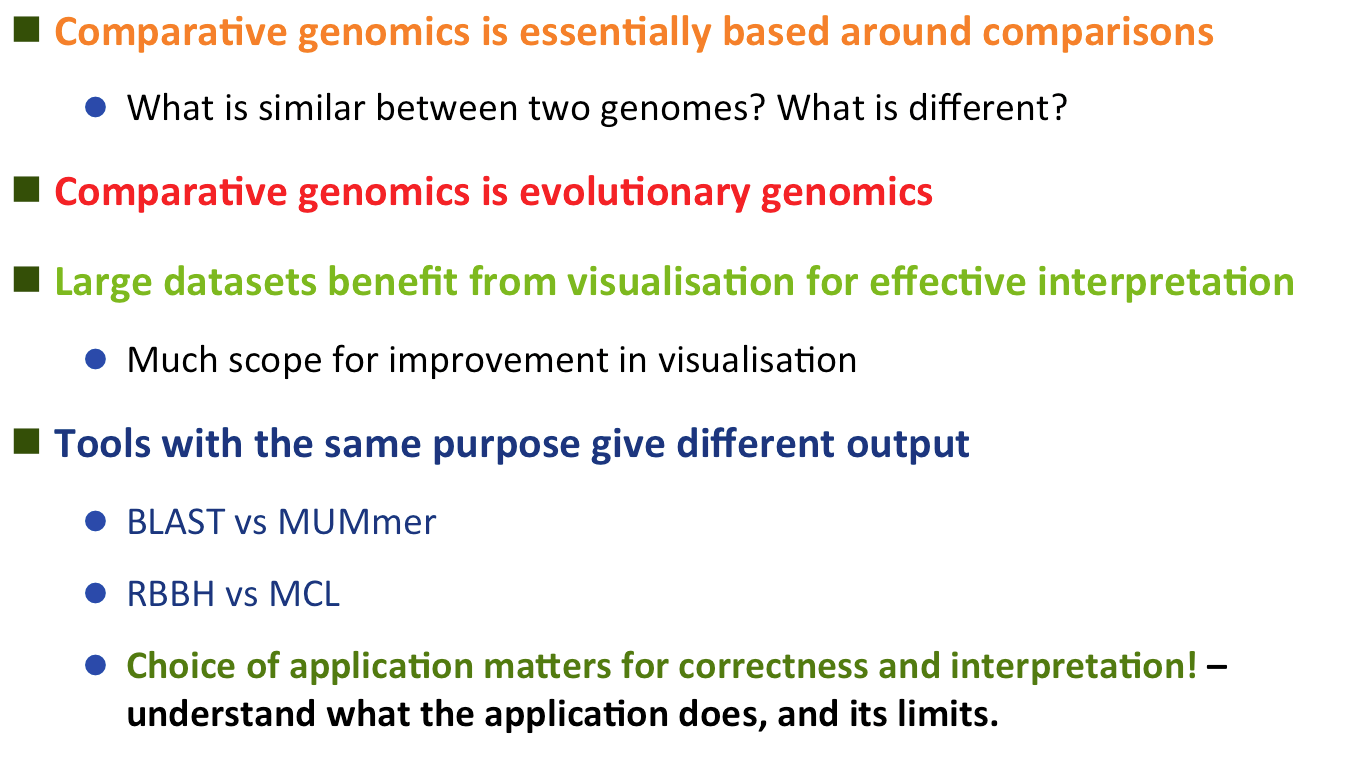
\includegraphics[width=1\textwidth]{images/conclusions2} 
  \end{center}
\end{frame}

% Which methods work best
\begin{frame}
  \frametitle{Conclusions}
  \begin{center}
      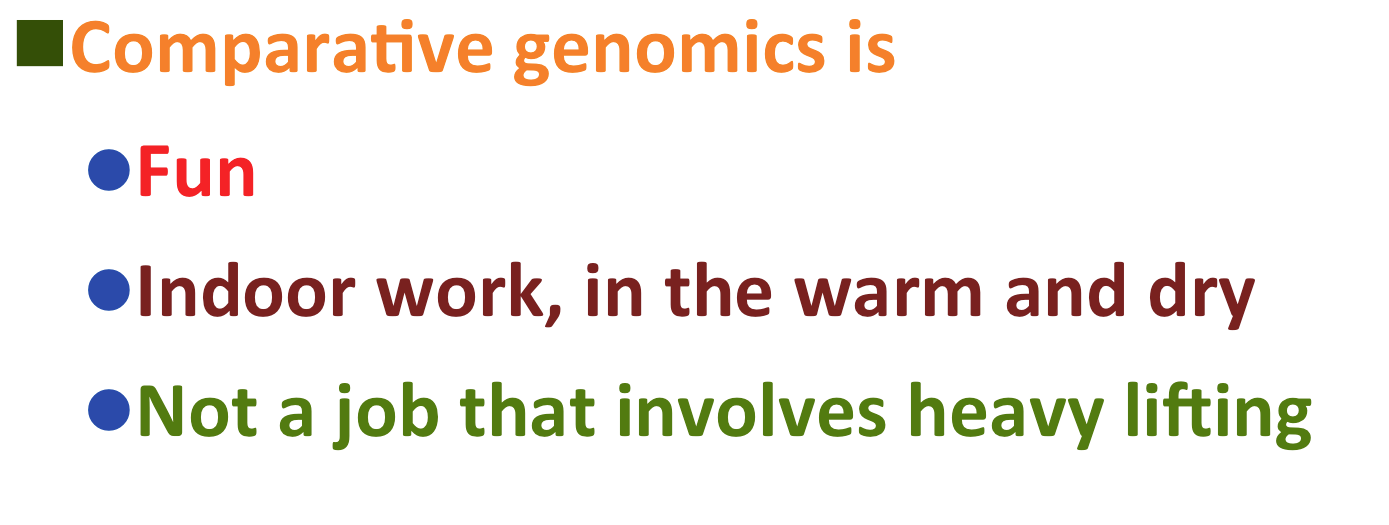
\includegraphics[width=1\textwidth]{images/conclusions3} 
  \end{center}
\end{frame}

%%%
% LICENCE FOR REUSE
%% licence.tex
%% Author: Leighton Pritchard
%% Copyright: James Hutton Institute
%% These slides describe the licence for reuse of these slides and
%% materials

%
\begin{frame}
  \frametitle{Licence: CC-BY-SA}
  By: Leighton Pritchard \\[0.5cm]
  This presentation is licensed under the Creative Commons Attribution ShareAlike license \\
  \href{https://creativecommons.org/licenses/by-sa/4.0/}{https://creativecommons.org/licenses/by-sa/4.0/}
\end{frame}

% etc
\end{document}